%%%%%%%%%%%%%%%%%%%%%%%%%%%%%%%%%%%%%%%%%
% baposter Landscape Poster
% LaTeX Template
% Version 1.0 (11/06/13)
%
% baposter Class Created by:
% Brian Amberg (baposter@brian-amberg.de)
%
% This template has been downloaded from:
% http://www.LaTeXTemplates.com
%
% License:
% CC BY-NC-SA 3.0 (http://creativecommons.org/licenses/by-nc-sa/3.0/)
%
%%%%%%%%%%%%%%%%%%%%%%%%%%%%%%%%%%%%%%%%%

%----------------------------------------------------------------------------------------
%	PACKAGES AND OTHER DOCUMENT CONFIGURATIONS
%----------------------------------------------------------------------------------------

\documentclass[landscape,a0paper,fontscale=0.285]{baposter} % Adjust the font scale/size here

\usepackage{graphicx} % Required for including images
\graphicspath{{figures/}} % Directory in which figures are stored

\usepackage{amsmath} % For typesetting math
\usepackage{amssymb} % Adds new symbols to be used in math mode

\usepackage{booktabs} % Top and bottom rules for tables
\usepackage{enumitem} % Used to reduce itemize/enumerate spacing
\usepackage{palatino} % Use the Palatino font
\usepackage[font=small,labelfont=bf]{caption} % Required for specifying captions to tables and figures

\usepackage{pgfplots}
\usepackage{pgfplotstable}
\usepackage{xcolor}

\usepackage{multicol} % Required for multiple columns
\setlength{\columnsep}{1.5em} % Slightly increase the space between columns
\setlength{\columnseprule}{0.2pt}
%\setlength{\columnseprule}{0mm} % No horizontal rule between columns

\usepackage{tikz} % Required for flow chart
\usetikzlibrary{shapes,arrows} % Tikz libraries required for the flow chart in the template

\newcommand{\compresslist}{ % Define a command to reduce spacing within itemize/enumerate environments, this is used right after \begin{itemize} or \begin{enumerate}
\setlength{\itemsep}{1pt}
\setlength{\parskip}{0pt}
\setlength{\parsep}{0pt}
}

\definecolor{arizonablue}{RGB}{21,36,74} % Defines the color used for content box headers

\definecolor{arizonared}{RGB}{171,5,32} % Defines the color used for content box headers


\begin{document}

\begin{poster}
{
headerborder=closed, % Adds a border around the header of content boxes
colspacing=1em, % Column spacing
bgColorOne=white, % Background color for the gradient on the left side of the poster
bgColorTwo=white, % Background color for the gradient on the right side of the poster
borderColor=arizonablue, % Border color
headerColorOne=arizonablue, % Background color for the header in the content boxes (left side)
headerColorTwo=arizonablue, % Background color for the header in the content boxes (right side)
headerFontColor=arizonared, % Text color for the header text in the content boxes
boxColorOne=white, % Background color of the content boxes
textborder=roundedleft, % Format of the border around content boxes, can be: none, bars, coils, triangles, rectangle, rounded, roundedsmall, roundedright or faded
eyecatcher=false, % Set to false for ignoring the left logo in the title and move the title left
headerheight=0.1\textheight, % Height of the header
headershape=roundedright, % Specify the rounded corner in the content box headers, can be: rectangle, small-rounded, roundedright, roundedleft or rounded
headerfont=\Large\bf\textsc, % Large, bold and sans serif font in the headers of content boxes
%textfont={\setlength{\parindent}{1.5em}}, % Uncomment for paragraph indentation
linewidth=2pt, % Width of the border lines around content boxes
columns=5
}
%----------------------------------------------------------------------------------------
%	TITLE SECTION 
%----------------------------------------------------------------------------------------
%
{
\includegraphics[height=4em]{ua_stack_rgb_4.pdf}} % First university/lab logo on the left
{\huge{\bf\textsc{Implementing and Testing:  Trimmed Serendipity Elements in Firedrake}\vspace{0.5em}}} % Poster title
{\textsc{Justin Crum$^1$, Cyrus Cheng$^2$, Joshua A. Levine$^1$, Robert Kirby$^3$, David Ham$^2$, Lawrence Mitchell$^4$, Andrew Gillette$^1$\\}
\small{$^1$ University of Arizona, $^2$ Imperial College, $^3$ Baylor University, $^4$Durham University} } % Author names and institution
{
\includegraphics[height=4em]{ua_stack_rgb_4.pdf}} % Second university/lab logo on the right

%----------------------------------------------------------------------------------------
%	OBJECTIVES
%----------------------------------------------------------------------------------------

\headerbox{Objectives}{name=objectives,column=0,row=0}{
Trimmed serendipity elements have rarely been implemented and tested in a comprehensive finite element method package.
 

\begin{enumerate}\compresslist
\item Implement trimmed serendipity elements in Firedrake
\item Test for correct convergence rates
\item Compare results against tensor product elements on a variety of test problems
\end{enumerate}

\vspace{0.3em} % When there are two boxes, some whitespace may need to be added if the one on the right has more content
}

%----------------------------------------------------------------------------------------
%	INTRODUCTION
%----------------------------------------------------------------------------------------

\headerbox{Introduction}{name=introduction,column=0,below=objectives, above=bottom}{
The trimmed serendipity finite elements \cite{gillette2019trimmed} are a family of finite elements that are used to approximate solutions to PDEs on square and cubical meshes.  We denote the family by $\mathcal{S}_r^- \Lambda^k$, where $r$ is the order of the element used and $k$ is the form degree.

%\begin{figure}[h]

\begin{center}
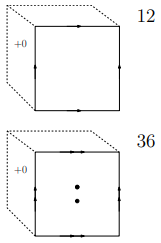
\includegraphics[width=0.4\textwidth]{trimmedSerendipityPT.PNG}

The above is an illustration of the degrees of freedom for trimmed serendipity elements, $\mathcal{S}_1^-\Lambda^1(\square_3)$ and $\mathcal{S}_2^-\Lambda^1(\square_3)$ .
\end{center}

One example of the set of edge basis functions for $\mathcal{S}_1^-\Lambda^1(\square_3)$, derived in \cite{gillette2019computational}, are:
\begin{equation*}
      (y\pm 1)(z\pm 1)dx + (x\pm 1)(z\pm 1) dy +
\end{equation*}
\begin{equation*}
    (x \pm 1)(y \pm 1)dz
\end{equation*}

where the proper choice of edge assignment will result in 12 different constant one forms.

}

%----------------------------------------------------------------------------------------
%	RESULTS 1
%----------------------------------------------------------------------------------------

%\headerbox{Results 1}{name=results,column=2,span=2,row=0,bottomaligned=introduction}{

%\begin{multicols}{2}
%\vspace{1em}
%\begin{center}
%\includegraphics[width=0.8\linewidth]{placeholder}
%\captionof{figure}{Figure caption}
%\end{center}

%Aliquam auctor, metus id ultrices porta, risus enim cursus sapien, quis iaculis sapien tortor sed odio. Mauris ante orci, euismod vitae tincidunt eu, porta ut neque. Aenean sapien est, viverra vel lacinia nec, venenatis eu nulla. Maecenas ut nunc nibh, et tempus libero. Aenean vitae risus ante. Pellentesque condimentum dui. Etiam sagittis purus non tellus tempor volutpat. Donec et dui non massa tristique adipiscing.
%\end{multicols}

%------------------------------------------------

%\begin{multicols}{2}
%%\vspace{1em}
%Sed fringilla tempus hendrerit. Vestibulum ante ipsum primis in faucibus orci luctus et ultrices posuere cubilia Curae; Etiam ut elit sit amet metus lobortis consequat sit amet in libero. Lorem ipsum dolor sit amet, consectetur adipiscing elit. Phasellus vel sem magna. Nunc at convallis urna. isus ante. Pellentesque condimentum dui. Etiam sagittis purus non tellus tempor volutpat. Donec et dui non massa tristique adipiscing. Quisque vestibulum eros eu.

%\begin{center}
%\includegraphics[width=0.8\linewidth]{placeholder}
%\captionof{figure}{Figure caption}
%\end{center}

%\end{multicols}
%}




%----------------------------------------------------------------------------------------
%	Firedrake
%----------------------------------------------------------------------------------------

\headerbox{Firedrake}{name=firedrake,column=1,span=3}{ % This block's bottom aligns with the bottom of the conclusion block
\begin{center}
    
\includegraphics[width=0.45\textwidth]{FiredrakeLogo.PNG}
\end{center}

In Firedrake \cite{rathgeber2016firedrake}, we are able to implement the trimmed serendipity finite elements by using the basis functions determined in \cite{gillette2019computational} and recreating the equation

\begin{equation}\label{eq:HCurlTrimmedSerendipityBasis}
   \mathcal{S}^-_r\Lambda^1(\square_3) =    \left[\bigoplus_{i=0}^{r-1} E_i \Lambda^1\right]\oplus\left[ \bigoplus_{i=2}^{r-1}F_i \Lambda^1\right] \oplus \left[\tilde{F}_r \Lambda^1\right]\oplus\left[ \bigoplus_{i=4}^{r-1}I_i \Lambda^1 \right] \oplus \left[\tilde{I}_r \Lambda^1\right]
   \end{equation}

inside of a FIAT element.  Then once a Firedrake code is asked to create a function space using
\begin{center}
{\fontfamily{qcr}\selectfont FunctionSpace(mesh, "SminusCurl", r)} \\
\end{center}
it chooses the appropriate set of basis functions based on what portions of Equation \ref{eq:HCurlTrimmedSerendipityBasis} need to be filled in for degree the chosen degree $r$.

}




%----------------------------------------------------------------------------------------
%	RESULTS
%----------------------------------------------------------------------------------------

\headerbox{Results}{name=results,column=1, span=3, below=firedrake, above=bottom}{

\begin{multicols}{3}
\begin{center}
\begin{tikzpicture}[scale=0.7]
      \begin{loglogaxis}[xlabel={Degrees of Freedom}, ylabel={Error},
             ylabel near ticks, ymax=1e-3, ymin=1e-11, xmax=2e8, xmin=1e3,
             legend pos=south west, legend style={font=\tiny} ,
             cycle list name=color list, title={Primal Poisson Error Analysis}]
        %\addplot+[only marks, orange] table [x=Dofs,y=Time,col sep=comma]{PrimalPoissonSerendipity3dO4.csv};
        \addplot[red]
        table [x=Dofs,y=Error, col sep=comma]{csvs/PrimalPoissonSerendipity3dO2.csv};
        \addlegendentry{$S^-_2$}
        \addplot[blue] 
        table [x=Dofs,y=Error, col sep=comma]{csvs/PrimalPoissonSerendipity3dO3.csv};
        \addlegendentry{$S^-_3$ }
        \addplot[orange]
        table [x=Dofs,y=Error, col sep=comma]{csvs/PrimalPoissonSerendipity3dO4.csv};
        \addlegendentry{$S^-_4$}
        \addplot[densely dotted, red]
        table [x=Dofs,y=Error, col sep=comma]{csvs/PrimalPoissonLagrange3dO2.csv};
        \addlegendentry{$Q^-_2$}
        \addplot[densely dotted, blue] 
        table [x=Dofs,y=Error, col sep=comma]{csvs/PrimalPoissonLagrange3dO3.csv};
        \addlegendentry{$Q^-_3$}
        \addplot[densely dotted, orange]
        table [x=Dofs,y=Error, col sep=comma]{csvs/PrimalPoissonLagrange3dO4.csv};
        \addlegendentry{$Q^-_4$}
        
        \addplot+[only marks, red] table [x=Dofs,y=Error,col sep=comma]{csvs/PrimalPoissonSerendipity3dO2.csv};
        \addplot+[only marks, red, mark=square*] table [x=Dofs,y=Error,col sep=comma]{csvs/PrimalPoissonLagrange3dO2.csv};
        \addplot+[only marks, blue] table [x=Dofs,y=Error,col sep=comma]{csvs/PrimalPoissonSerendipity3dO3.csv};
        \addplot+[only marks, blue, mark=square*] table [x=Dofs,y=Error,col sep=comma]{csvs/PrimalPoissonLagrange3dO3.csv};
        \addplot+[only marks, orange] table [x=Dofs,y=Error,col sep=comma]{csvs/PrimalPoissonSerendipity3dO4.csv};
        \addplot+[only marks, orange, mark=square*] table [x=Dofs,y=Error,col sep=comma]{csvs/PrimalPoissonLagrange3dO4.csv};
      \end{loglogaxis}
      \end{tikzpicture}
      
\begin{tikzpicture}[scale=0.7]
      \begin{loglogaxis}[xlabel={Time}, ylabel={Error},
             ylabel near ticks, ymax=1e-3, ymin=1e-11, xmax=1e4, xmin=0.5e-1,
             legend pos=north east, legend style={font=\tiny} ,
             cycle list name=color list, title={Primal Poisson Time Analysis}]
        %\addplot+[only marks, orange] table [x=Dofs,y=Time,col sep=comma]{PrimalPoissonSerendipity3dO4.csv};
        \addplot[red]
        table [x=Time,y=Error, col sep=comma]{csvs/PrimalPoissonSerendipity3dO2.csv};
        \addlegendentry{$S^-_2$}
        \addplot[blue] 
        table [x=Time,y=Error, col sep=comma]{csvs/PrimalPoissonSerendipity3dO3.csv};
        \addlegendentry{$S^-_3$ }
        \addplot[orange]
        table [x=Time,y=Error, col sep=comma]{csvs/PrimalPoissonSerendipity3dO4.csv};
        \addlegendentry{$S^-_4$}
        \addplot[densely dotted, red]
        table [x=Time,y=Error, col sep=comma]{csvs/PrimalPoissonLagrange3dO2.csv};
        \addlegendentry{$Q^-_2$}
        \addplot[densely dotted, blue] 
        table [x=Time,y=Error, col sep=comma]{csvs/PrimalPoissonLagrange3dO3.csv};
        \addlegendentry{$Q^-_3$}
        \addplot[densely dotted, orange]
        table [x=Time,y=Error, col sep=comma]{csvs/PrimalPoissonLagrange3dO4.csv};
        \addlegendentry{$Q^-_4$}
        
        \addplot+[only marks, red] table [x=Time,y=Error,col sep=comma]{csvs/PrimalPoissonSerendipity3dO2.csv};
        \addplot+[only marks, red, mark=square*] table [x=Time,y=Error,col sep=comma]{csvs/PrimalPoissonLagrange3dO2.csv};
        \addplot+[only marks, blue] table [x=Time,y=Error,col sep=comma]{csvs/PrimalPoissonSerendipity3dO3.csv};
        \addplot+[only marks, blue, mark=square*] table [x=Time,y=Error,col sep=comma]{csvs/PrimalPoissonLagrange3dO3.csv};
        \addplot+[only marks, orange] table [x=Time,y=Error,col sep=comma]{csvs/PrimalPoissonSerendipity3dO4.csv};
        \addplot+[only marks, orange, mark=square*] table [x=Time,y=Error,col sep=comma]{csvs/PrimalPoissonLagrange3dO4.csv};
     \end{loglogaxis}
\end{tikzpicture}

\begin{tikzpicture}[scale=0.7]
      \begin{loglogaxis}[xlabel={Degrees of Freedom}, ylabel={Error},
             ylabel near ticks, ymax=1.2e-2, ymin=0.8e-7, xmax=2e7, xmin=5e3,
             legend pos=south west, legend style={font=\tiny} ,
             cycle list name=color list, title={Mixed Poisson Error Analysis}]
        %\addplot+[only marks, orange] table [x=Dofs,y=Time,col sep=comma]{PrimalPoissonSerendipity3dO4.csv};
        \addplot[red]
        table [x=Dofs,y=Error, col sep=comma]{csvs/MixedPoissonSminus3dO2.csv};
        \addlegendentry{$S^-_2$}
        \addplot[blue] 
        table [x=Dofs,y=Error, col sep=comma]{csvs/MixedPoissonSminus3dO3.csv};
        \addlegendentry{$S^-_3$ }
        \addplot[orange]
        table [x=Dofs,y=Error, col sep=comma]{csvs/MixedPoissonSminus3dO4.csv};
        \addlegendentry{$S^-_4$}
        \addplot[densely dotted, red]
        table [x=Dofs,y=Error, col sep=comma]{csvs/MixedPoissonNCF3dO2.csv};
        \addlegendentry{$Q^-_2$}
        \addplot[densely dotted, blue] 
        table [x=Dofs,y=Error, col sep=comma]{csvs/MixedPoissonNCF3dO3.csv};
        \addlegendentry{$Q^-_3$}
        \addplot[densely dotted, orange]
        table [x=Dofs,y=Error, col sep=comma]{csvs/MixedPoissonNCF3dO4.csv};
        \addlegendentry{$Q^-_4$}
        
        \addplot+[only marks, red] table [x=Dofs,y=Error,col sep=comma]{csvs/MixedPoissonSminus3dO2.csv};
        \addplot+[only marks, red, mark=square*] table [x=Dofs,y=Error,col sep=comma]{csvs/MixedPoissonNCF3dO2.csv};
        \addplot+[only marks, blue] table [x=Dofs,y=Error,col sep=comma]{csvs/MixedPoissonSminus3dO3.csv};
        \addplot+[only marks, blue, mark=square*] table [x=Dofs,y=Error,col sep=comma]{csvs/MixedPoissonNCF3dO3.csv};
        \addplot+[only marks, orange] table [x=Dofs,y=Error,col sep=comma]{csvs/MixedPoissonSminus3dO4.csv};
        \addplot+[only marks, orange, mark=square*] table [x=Dofs,y=Error,col sep=comma]{csvs/MixedPoissonNCF3dO4.csv};
      \end{loglogaxis}
      \end{tikzpicture}
      
      
    \begin{tikzpicture}[scale=0.7]
      \begin{loglogaxis}[xlabel={Time}, ylabel={Error},
             ylabel near ticks, ymax=1e-1, ymin=5e-8, xmax=1e5, xmin=0.5e-1,
             legend pos=north east, legend style={font=\tiny} ,
             cycle list name=color list, title={Mixed Poisson Time Analysis}]
        %\addplot+[only marks, orange] table [x=Dofs,y=Time,col sep=comma]{PrimalPoissonSerendipity3dO4.csv};
        \addplot[red]
        table [x=Time,y=Error, col sep=comma]{csvs/MixedPoissonSminus3dO2.csv};
        \addlegendentry{$S^-_2$}
        \addplot[blue] 
        table [x=Time,y=Error, col sep=comma]{csvs/MixedPoissonSminus3dO3.csv};
        \addlegendentry{$S^-_3$ }
        \addplot[orange]
        table [x=Time,y=Error, col sep=comma]{csvs/MixedPoissonSminus3dO4.csv};
        \addlegendentry{$S^-_4$}
        \addplot[densely dotted, red]
        table [x=Time,y=Error, col sep=comma]{csvs/MixedPoissonNCF3dO2.csv};
        \addlegendentry{$Q^-_2$}
        \addplot[densely dotted, blue] 
        table [x=Time,y=Error, col sep=comma]{csvs/MixedPoissonNCF3dO3.csv};
        \addlegendentry{$Q^-_3$}
        \addplot[densely dotted, orange]
        table [x=Time,y=Error, col sep=comma]{csvs/MixedPoissonNCF3dO4.csv};
        \addlegendentry{$Q^-_4$}
        
        \addplot+[only marks, red] table [x=Time,y=Error,col sep=comma]{csvs/MixedPoissonSminus3dO2.csv};
        \addplot+[only marks, red, mark=square*] table [x=Time,y=Error,col sep=comma]{csvs/MixedPoissonNCF3dO2.csv};
        \addplot+[only marks, blue] table [x=Time,y=Error,col sep=comma]{csvs/MixedPoissonSminus3dO3.csv};
        \addplot+[only marks, blue, mark=square*] table [x=Time,y=Error,col sep=comma]{csvs/MixedPoissonNCF3dO3.csv};
        \addplot+[only marks, orange] table [x=Time,y=Error,col sep=comma]{csvs/MixedPoissonSminus3dO4.csv};
        \addplot+[only marks, orange, mark=square*] table [x=Time,y=Error,col sep=comma]{csvs/MixedPoissonNCF3dO4.csv};
      \end{loglogaxis}
      \end{tikzpicture}
      

\begin{tikzpicture}[scale=0.7]
      \begin{loglogaxis}[xlabel={Dofs}, ylabel={Error},
             ylabel near ticks, ymax=1e-3, ymin=1e-14, xmax=3e6, xmin=3.5e4,
             legend pos=north east, legend style={font=\tiny} ,
             cycle list name=color list, title={Maxwell Eigenvalue Analysis}]
        %\addplot+[only marks, orange] table [x=Dofs,y=Time,col sep=comma]{PrimalPoissonSerendipity3dO4.csv};
        \addplot[green, mark=diamond]
        table [x=Dofs,y=Error, col sep=comma]{csvs/SminusEigenvaluesValue3.csv};
        \addlegendentry{$S^- \lambda = 3$}
        \addplot[densely dotted, green, mark=square*]
        table [x=Dofs,y=Error, col sep=comma]{csvs/TensorEigenvaluesValue3.csv};
        \addlegendentry{$Q^- \lambda = 3$}
        \addplot[violet, mark=diamond] 
        table [x=Dofs,y=Error, col sep=comma]{csvs/SminusEigenvaluesValue5.csv};
        \addlegendentry{$S^- \lambda = 5$ }
        \addplot[densely dotted, violet, mark=square*]
        table [x=Dofs,y=Error, col sep=comma]{csvs/TensorEigenvaluesValue5.csv};
        \addlegendentry{$Q^- \lambda = 5$}

        
        %\addplot+[only marks, red] table [x=Dofs,y=Error,col sep=comma]{csvs/SminusEigenvaluesValue3.csv};
        %\addplot+[only marks, red, mark=square*] table [x=Dofs,y=Error,col sep=comma]{csvs/TensorEigenvaluesValue3.csv};
        %\addplot+[only marks, blue] table [x=Dofs,y=Error,col sep=comma]{csvs/SminusEigenvaluesValue5.csv};
        %\addplot+[only marks, blue, mark=square*] table [x=Dofs,y=Error,col sep=comma]{csvs/TensorEigenvaluesValue5.csv};
      \end{loglogaxis}
      \end{tikzpicture}

      
      
\begin{tikzpicture}[scale=0.7]
      \begin{loglogaxis}[xlabel={Time}, ylabel={Error},
             ylabel near ticks, ymax=1e-3, ymin=1e-14, xmax=185, xmin=0,
             legend pos=north east, legend style={font=\tiny} ,
             cycle list name=color list, title={Maxwell Eigenvalue Analysis}]
        %\addplot+[only marks, orange] table [x=Dofs,y=Time,col sep=comma]{PrimalPoissonSerendipity3dO4.csv};
        \addplot[green, mark=diamond]
        table [x=Time,y=Error, col sep=comma]{csvs/SminusEigenvaluesValue3.csv};
        \addlegendentry{$S^- \lambda = 3$}
        \addplot[densely dotted, green, mark=square*]
        table [x=Time,y=Error, col sep=comma]{csvs/TensorEigenvaluesValue3.csv};
        \addlegendentry{$Q^- \lambda = 3$}
        \addplot[violet, mark=diamond] 
        table [x=Time,y=Error, col sep=comma]{csvs/SminusEigenvaluesValue5.csv};
        \addlegendentry{$S^- \lambda = 5$ }
        \addplot[densely dotted, violet, mark=square*]
        table [x=Time,y=Error, col sep=comma]{csvs/TensorEigenvaluesValue5.csv};
        \addlegendentry{$Q^- \lambda = 5$}

        
        %\addplot+[only marks, green, mark=circle*] table [x=Time,y=Error,col sep=comma]{csvs/SminusEigenvaluesValue3.csv};
        %\addplot+[only marks, green, mark=square*] table [x=Time,y=Error,col sep=comma]{csvs/TensorEigenvaluesValue3.csv};
        %\addplot+[only marks, purple, mark=circle] table [x=Time,y=Error,col sep=comma]{csvs/SminusEigenvaluesValue5.csv};
        %\addplot+[only marks, purple, mark=square] table [x=Time,y=Error,col sep=comma]{csvs/TensorEigenvaluesValue5.csv};
      \end{loglogaxis}
      \end{tikzpicture}
      

\end{center}
\end{multicols}
}

%----------------------------------------------------------------------------------------


%----------------------------------------------------------------------------------------
%	Discussion
%----------------------------------------------------------------------------------------

\headerbox{Discussion}{name=discussion,column=4}{ 

The primal Poisson and mixed Poisson error analysis graphs illustrate that $\mathcal{S}^-_r$ elements are converging at the expected rates, and that there are scenarios where either the $\mathcal{S}^-_r$ or $\mathcal{Q}^-_r$ elements might be useful.  The timing data below both of these error analysis plots also enforces this. \\

The Maxwell Eigenvalue problem illustrates one example where using trimmed serendipity elements might be able to save researchers a lot of time at a relatively small loss in error.  Results here are found by using SLEPc inside of Firedrake, and calling the {\fontfamily{qcr}\selectfont  "SminusCurl"} or {\fontfamily{qcr}\selectfont  "NCE"} families.



}

%----------------------------------------------------------------------------------------


%----------------------------------------------------------------------------------------
%	Future Works
%----------------------------------------------------------------------------------------

\headerbox{Future Work}{name=future,column=4, below=discussion}{ 
In the future we would like to do:

\begin{enumerate}\compresslist
    \item Test trimmed serendipity elements on specific application contexts 
    \item Implement regular serendipity elements
    %\item Further investigate uses of trimmed serendipity elements as a route for solution refinement
\end{enumerate}


}

%----------------------------------------------------------------------------------------



%----------------------------------------------------------------------------------------
%	REFERENCES
%----------------------------------------------------------------------------------------

\headerbox{References}{name=references,column=4,below=future}{


\renewcommand{\section}[2]{\vskip 0.05em} % Get rid of the default "References" section title
\nocite{*} % Insert publications even if they are not cited in the poster
\tiny{% Reduce the font size in this block
\bibliographystyle{abbrv}
\bibliography{poster} % Use sample.bib as the bibliography file

}}


%----------------------------------------------------------------------------------------
%	Acknowledgements
%----------------------------------------------------------------------------------------

\headerbox{Acknowledgements}{name=acknowledgements,column=4, below=references, above=bottom}{ 

Research supported in part by NSF Collaborative Research Award DMS-1913094 and DMS-1912653.
\begin{center}

\includegraphics[scale=0.15]{nsf.pdf}
\end{center}
}

%----------------------------------------------------------------------------------------





\end{poster}

\end{document}